\chapter[Lecture 21]{}\label{lec21}

At high temperature, all phonon modes are excited, because $k_{B}T>\hbar w_{\max}$. Therefore substantial portion of phonon collisions will be Umklapp process and one can neglect distinction between normal process and Umklapp process.

Thermal resistivity $\alpha_{i}T$ at high Temperature.

Al low temperature Umklapp to occur, one needs to have $k_{1}$, $k_{2}$ of the order $\dfrac{1}{2}k_{B}\theta$ at least as each phonon must have wave vector $\dfrac{1}{2}G$ to bring in consideration of $G$.

Following Boltzmann distance this no. $\sim e^{-\frac{\theta}{2T}}$

$\therefore \ $ Collision will be $\sim e^{-\frac{\theta}{2T}}$

mean free path depends on {\em Umklapp}.

Periodic potential in a solid
\begin{figure}[H]
\centering
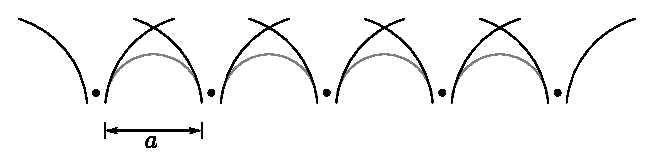
\includegraphics{images/lecture21/fig1.eps}
\end{figure}

Potential energy
$$
v(x+na)=u(x)
$$
wave for $\psi(x+na)=\phi(x)$, $n=$ integer.

Bloch's Theorem \fbox{$\psi_{k}(r)=u_{k}(r)e^{ikr}$}

$k\to$ reciprocal lattice vector.

Comes purely from the translational symmetry considerations.
\begin{itemize}
\item[(i)] Electrons close to the nucleus will behave like atomic orbitals as the influence of potential from other sites is small.

\item[(ii)] Electrons in the out most orbitals are most exposed to the crystal lattice potential.

\item[(iii)] Inner electrons screens the positive potential of the nucleus significantly. Depends strongly on orbitals.
\end{itemize}

$d$ and $f$ (complex) shells are different from $s$ and $p$ (spherical symm.) shells.

Simplest model to capture the lattice effect is

\section*{Kromg-Penney model}

Assume the lattice as a square well potential.
\begin{figure}[H]
\centering
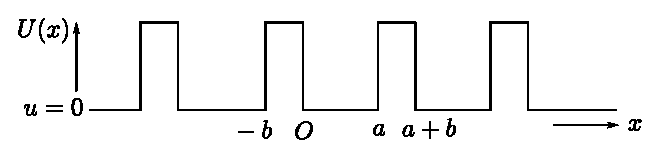
\includegraphics{images/lecture21/fig2.eps}
\end{figure}
\begin{align*}
\dfrac{Q^{2}-k^{2}}{2Qk}\sin h \ Qb \sin Ka+\cos \Delta Qb \cos Ka &= \cos k(a+b)\\
Q^{2} &= \dfrac{2p}{ab}
\end{align*}
\begin{align*}
\Rightarrow\quad & \dfrac{Q}{2K}\sin h \ Qb\sin Ka+\cos Ka = \cos ka\\[3pt]
& \dfrac{Q^{2}b}{2K}\sin Ka +\cos Ka = \cos ka\\[3pt]
\Rightarrow & \fbox{$\dfrac{P}{Ka}\sin Ka+\cos Ka = \cos Ka$}
\end{align*}
Schr\"odinger equation
$$
-\dfrac{\hbar^{2}}{2m}\dfrac{d^{2}\psi}{dx^{2}}+U(x)\psi = \epsilon \psi
$$
at $0<x<a$\quad $U=0$
\begin{align*}
\therefore\quad \psi &= \Delta e^{iKx}+Be^{-iKx}\\
\epsilon &= \dfrac{\hbar^{2}K^{2}}{2m}
\end{align*}
$-b<x<0$\quad $\psi(x)=Ce^{Q_{x}}+De^{-Qx}$ as $U=U_{0}$
$$
\therefore\quad U_{0}-\epsilon = \dfrac{\hbar^{2}Q^{2}}{2M}
$$
Since the potential is periodic with periodicity $(a+b)$
$$
\psi(a<x<a+b)=\psi(-b<x<0)e^{ik(a+b)}
$$
$\therefore$ To determine $A$, $B$, $C$, $D$, one can use a boundary condition
\begin{quote}
$\psi(x)$ is continuous at $x=0$ and $x=a$

$\psi'(x)$ is continuous at $x=0$ and $x=a$.
\end{quote}
$\therefore$ The four equations are
\begin{gather*}
\left.
\begin{array}{c}
A+B=C+D\\
iK(A-B)=Q(C-D)
\end{array}
\right\} \quad \text{at } x=0\\[4pt]
\left.
\begin{array}{c}
Ae^{ika}+Be^{-ika}=(Ce^{-Qb}+De^{+Qb})e^{ik(a+b)}\\[2pt]
iK (Ae^{iKa}-Be^{-ika})=Q(Ce^{-Qb}-De^{Qb})e^{ik(a+b)}
\end{array}
\right\}\quad x=0
\end{gather*}
shifted by $(a+b)$.

To have a solution determinant of the co-efficients of $A$, $B$, $C$, $D$ should vanish. From that one finds.
$$
[(Q^{2}-K^{2})/2Qk]\sin Ka \sin h \ Qb+\cos Ka \cos h \ Qb = \cos k(a+b)
$$
To get a simplified solution assume $b\to 0$ and $U_{0}\to \infty$ in such a way that \fbox{$Q^{2}ba/2=P$}, a finite quantity.
$$
\Rightarrow Q\gg K\quad \text{and}\quad Qb\ll 1
$$
$\therefore \ $ The solution becomes,
$$
\fbox{$\dfrac{P}{Ka}\sin Ka + \cos Ka=\cos Ka$}
$$
\begin{figure}[H]
\centering
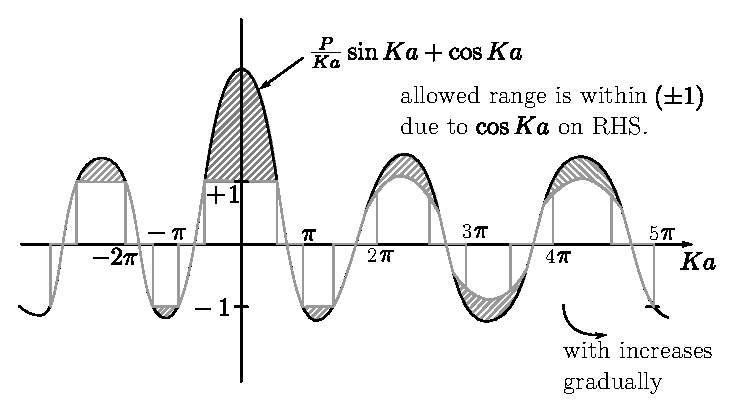
\includegraphics[scale=.9]{images/lecture21/fig3.eps}
\end{figure}

$\epsilon = \dfrac{\hbar^{\nu}K^{\nu}}{2m}\Rightarrow$ Allowed values of $\epsilon$ are given by the range of \fbox{$Ka=\sqrt{\dfrac{2m\epsilon}{\hbar^{2}}}\cdot a$} for which the function lies between $(\pm 1)$.

Solutions for other value of $Ka$ are not allowed $\to$ forbidden gap.
\begin{figure}[H]
\centering
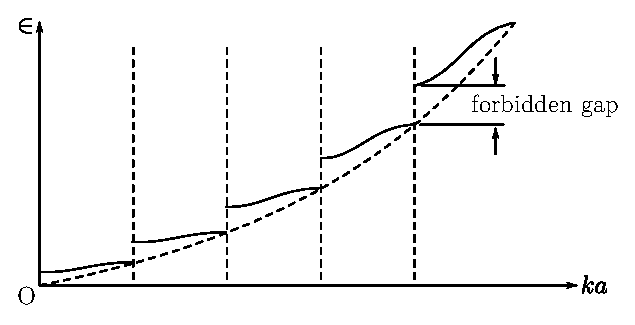
\includegraphics[scale=.9]{images/lecture21/fig4.eps}
\end{figure}

\section*{A General Solution}

Following Bloch Theorem, the potential function can be written as $U(x)=U(x+a)$.

$\therefore$ The potential felt by a state at $x$ is
$$
U(x)=\sum\limits_{G}U_{G}e^{iGx}\quad G\to \text{reciprocal lattice vector.}
$$
$\therefore$ The Schrodinger equation $H\psi=\epsilon\psi$ can be written as
$$
\left(\dfrac{P^{2}}{2m}+\sum\limits_{G}U_{G}e^{iGx}\right)\psi(x)=\epsilon\psi(x)
$$
The Bloch function $\psi(x)$ is $\psi(x)=\sum\limits_{k}C(k)e^{ikx} \ k=\dfrac{2\pi n}{L} \ C(k)\to C_{k}(x)$ a function of $k$ and $x$.
$$
p =-i\hbar^{2}\dfrac{d^{2}}{dx^{2}}\quad \therefore\quad \dfrac{P^{2}}{2m}\psi(x) =\dfrac{\hbar^{2}}{2m}\sum\limits_{k}C(k)\cdot k^{2}e^{ikx}
$$
The wave equation becomes
$$
\sum\limits_{k}\hbar^{2}_{2m}k^{2}C(k)e^{ikx}+\sum\limits_{G,k}U_{G}C(k)e^{i(k+G)x}=\epsilon \sum\limits_{k}C(k)e^{ikx}
$$
Each fourier component must have same co-efficient on both sides.
$$
\therefore\quad \fbox{$(\lambda_{k}-\epsilon)C(k)+\sum\limits_{G}U_{G}C(k-G)=0$}
$$
$\lambda_{k}=\dfrac{\hbar^{2}k^{2}}{2m}$. This is the central equation.

The equation looks simple but formidable to solve as there are infinite no. of $C(k-G)$. Usually, only few works well (two or four).

In an atom, $l$ and $m$ are two quantum no.s related to spherical symmetry. In solid, spherical symmetry is broken and there is a translational symmetry $\to k$. $\therefore \ k$ can be viewed as a quantum number. It has two interpretation (i) a wave vector for a Block wave or (ii) a quantum number describing the state of an electron in solid.

Remember, $\hbar k$ is not the momentum of a Bloch wave, the state does not change even if $k$ changes by a lattice translation vector, $G$.

Once $C$'s are determined, one can find the wave functions as
\begin{align*}
\psi_{k}(x) &= \sum\limits_{G}C(k-G)e^{i(k-G)x}\\
&= \left(\sum\limits_{G}C(k-G)e^{-iGx}\right)\cdot e^{ikx}\\
&= \mu_{k}(x)\cdot e^{ikx}\quad \fbox{$\mu_{kx}(x)=\sum\limits_{G}C(k-G)e^{-iGx}$}
\end{align*}
\begin{itemize}
\item[(i)] $u_{k}(x)$ is Fourier series over the reciprocal lattice and hence invariant under lattice translation
$$
u_{k}(x+T)=u_{k}(x)
$$

\item[(ii)] If lattice potential vanishes, then $(\lambda_{k}-\epsilon)C(k)=0$

$\therefore$ All $C(k-G)=0$ except $C(k)\Rightarrow u_{k}(x)=$ Const.

$\therefore \ \psi(x)\simeq e^{ikx}\to$ free particle.

\item[(iii)] $\hbar k\to$ crystal momentum of an electron

electron-phonon scattering $k+q \text{ (phonon momentum) } = k'+G$

electron at a state $k$ absorbs a phonon of wave vector $q$ and get scattered to $k'$ with reciprocal lattice vector $G$.
\end{itemize}

\section*{Nearly free electron approximation}

Lets assume, the electrons in the outermost orbital are very similar like free electrons.
$$
\therefore\quad \epsilon_{k}=\dfrac{\hbar^{2}k^{2}}{2m}
$$

Since all the distinct $k$ points are captured within the first Brillouin zone, one should move all the energies outside within the first zone using \fbox{$k'+G=k$}.

Since the energies and corresponding significant $k$ do not change by this translation in reciprocal space. $k'\equiv k$
\begin{align*}
\therefore\quad \epsilon_{k} &= \dfrac{\hbar^{2}(k+G)^{2}}{2m}\\
&= \dfrac{\hbar^{2}}{2m}\left[(k_{x}+G_{x})^{2}+(k_{y}+G_{y})^{2}+(k_{z}+G_{z})^{2}\right]
\end{align*}
\begin{figure}[H]
\centering
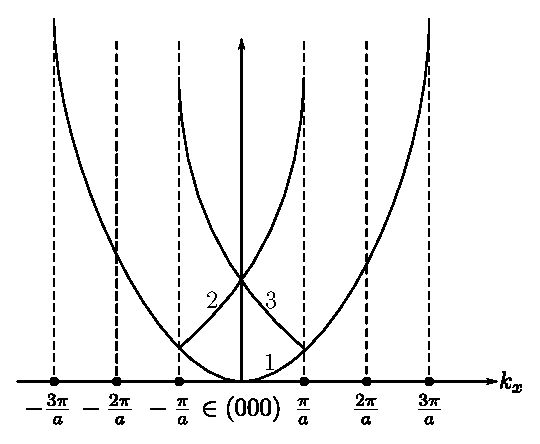
\includegraphics{images/lecture21/fig5.eps}
\end{figure}
\begin{center}
\begin{tabular}{cccc}
\hline
{\bf Band} & {\boldmath$G$} & {\boldmath$\epsilon(000)$} & {\boldmath$\epsilon(k_{x}00)$}\\
\hline
1 & 000 & 000 & $k^{2}_{x}$\\
$2,3$ & $(100)(T00)$ & $(2\pi/a)^{2}$ & $\left(k_{x}\pm \dfrac{2\pi}{a}\right)^{2}$\\
\hline
\end{tabular}
\end{center}
This comes purely from periodicity.

If the Fourier components, $U_{G}$ are small in comparison to the kinetic energy of electrons $\to$ Lets calculate the effect of $U_{G}$ on bands.
$$
at \ k_{x}=\pm \dfrac{\pi}{a}\quad k^{2}=\left(\dfrac{G}{2}\right)^{2}\quad (k-G)^{2}=\left(\dfrac{G}{2}\right)^{2}
$$
In, $\psi_{k}(x)=\sum\limits_{G}C(k-G)e^{i(k-G)x}$, $C\left(\dfrac{G}{2}\right)$ and $C\left(-\dfrac{G}{2}\right)$ are important at $k=\pm \dfrac{\pi}{a}=\pm \dfrac{G}{2}$.

So, we ignore all other co-efficients.

$\therefore$ The central equation 
\begin{equation*}
(\lambda_{k}-\epsilon)C(k)+\sum\limits_{G}U_{G}C(k-G)=0\tag{A}\label{lec21-eqA}
\end{equation*}
At $k=\dfrac{G}{2} \ \lambda = \dfrac{\hbar^{2}}{2m}\left(\dfrac{G}{2}\right)^{2}$

From \eqref{lec21-eqA}
\begin{equation*}
(\lambda-\epsilon)C(G/2)+UC(-G/2)=0\tag{1}\label{lec21-eq1}
\end{equation*}

At $k=G/2$ that is generated by shifting $k=-\dfrac{G}{2}$ by $G$
\begin{equation*}
(\lambda-\epsilon)C(-G/2)+UC(G/2)=0\tag{2}\label{lec21-eq2}
\end{equation*}

For non-trivial solution of equations \eqref{lec21-eq1} and \eqref{lec21-eq2}
$$
\left|
\begin{array}{cc}
\lambda-\epsilon & U\\
U & \lambda-\epsilon
\end{array}
\right|=0
$$
or,
\begin{align*}
\epsilon &= \lambda\pm U\\
&= \dfrac{\hbar^{2}G^{2}}{8m}\pm U=\epsilon^{\pm}
\end{align*}
The energy has two roots : one lower than $\lambda$ and the other higher than $\lambda$ at the zone boundary.

From equation \eqref{lec21-eq1} 
$$
\dfrac{C\left(-\frac{1}{2}G\right)}{C\left(\frac{G}{2}\right)}=\dfrac{\epsilon-\lambda}{\nu}=\pm 1
$$
$\therefore$ Fourier expansion of $\psi(x)$ has two solutions at the zone boundary 
\begin{align*}
& \psi(x)=e^{(iGx/2)}\pm e^{-(iGx/2)}\\
&\text{(+ve) sign for } \epsilon=\lambda+U\\
&\text{(-ve) sign for } \epsilon=\lambda-V
\end{align*}
For a general $k$ near the zone-boundary
$$
\psi(x)=C(k)e^{ikx}+C(k-G)e^{-k(k-G)x}\text{ from central equation}
$$
$\therefore$ The two equations from central equation will be
\begin{align*}
& (\lambda_{k}-\epsilon)C(k)+UC(k-G)=0\\
& (\lambda_{k-G}-\epsilon)C(k-G)+UC(k)=0
\end{align*}
To have a solution
$$
\left|
\begin{array}{cc}
\lambda_{k}-\epsilon & U\\
U & \lambda_{k-G}-\epsilon
\end{array}
\right|=0
$$
\begin{gather*}
\dfrac{\hbar^{2}k^{2}}{2m}+\dfrac{\hbar^{2}(k-G)^{2}}{2m}=\dfrac{\hbar^{2}}{2m}\left[\left(\widetilde{K}+\dfrac{G}{2}\right)^{2}+\left(\widetilde{K}-\dfrac{G}{2}\right)^{2}\right]=\dfrac{\hbar^{2}}{2m}\left[\widetilde{K}^{2}+\dfrac{G^{2}}{4}\right]\\
\therefore\quad \epsilon^{2}-\epsilon (\lambda_{k-G}+\lambda_{k})+\lambda_{k-G}\lambda_{k}-U^{2}=0\\
a, \epsilon=\dfrac{1}{2}(\lambda_{k-G}+\lambda_{k})\pm \left[\frac{1}{4}(\lambda_{k-G}-\lambda_{k})^{2}+U^{2}\right]^{\frac{1}{2}}
\end{gather*}
If we write $\widetilde{K}=k-G/2$; the difference between $k$ and zone boundary
\begin{align*}
\epsilon_{k} &= \dfrac{\hbar^{2}}{2m}\left(G^{2}/4+\widetilde{K}^{2}\right)\pm \left[4\lambda \dfrac{\hbar^{2}\widetilde{K}^{2}}{2m}+U^{2}\right]^{\frac{1}{2}}\\
&\simeq \dfrac{\hbar^{2}}{2m}\left(G^{2}/4+\widetilde{K}^{2}\right)\pm U \left[1+2(\lambda/U^{2})\dfrac{\hbar^{2}\widetilde{K}^{2}}{2m}\right]\\
&= \epsilon^{\pm}+\dfrac{\hbar^{2}\widetilde{K}^{2}}{2m}\left(1\pm \dfrac{2\lambda}{U}\right)
\end{align*}
\fbox{$U \text{ is (-ve)} \sim -0.45$}
\begin{figure}[H]
\centering
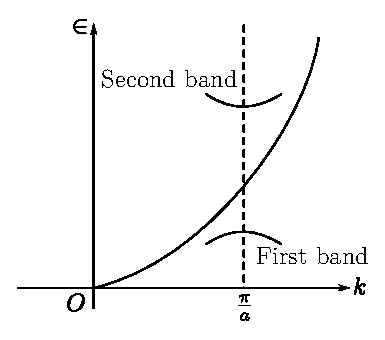
\includegraphics{images/lecture21/fig6.eps}
\end{figure}

\noindent
{\bf First band}
$$
\epsilon_{k}=\epsilon^{+}+\dfrac{\hbar^{2}\widetilde{K}^{2}}{2m}\left(1+\dfrac{2\lambda}{U}\right)
$$
{\bf Second band}
$$
\epsilon_{k}=\epsilon^{-}\pm \dfrac{\hbar^{2}\widetilde{K}^{2}}{2m}\left(1-\dfrac{2\lambda}{U}\right)
$$
symmetric at the zone boundary
$$
\text{Derivative, } \dfrac{d\epsilon}{dk}=0
$$
\begin{figure}[H]
\centering
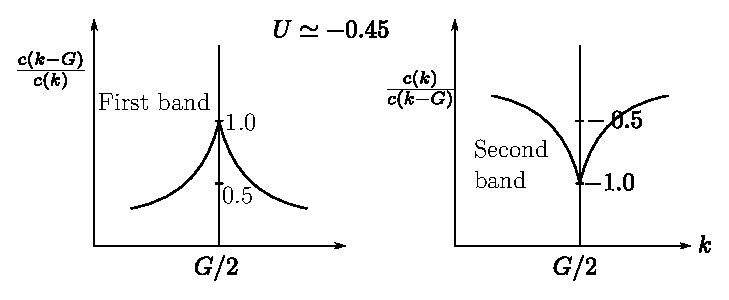
\includegraphics{images/lecture21/fig7.eps}
\end{figure}

\section*{No. of orbitals in a band}

For a one dimensional lattice of length $L$ and Lattice count `$a$' $k=0$, $\pm \dfrac{2\pi}{L}$, $\pm \dfrac{4\pi}{L},\ldots,\dfrac{N\pi}{L}$. $L=Na$ $N=$ no. of atoms.

$-\dfrac{N\pi}{L}$ is not considered as it is connected to $\dfrac{N\pi}{2}=\dfrac{\pi}{a}$

$\therefore$ Total No. of distinct $k$ values $=N$.

